\chapter{特征融合及RLCCD框架验证}
\label{chap:fusion}
本章主要对RLCCD方法中最后一环:基于多模态学习的特征融合方法进行介绍,同时针对RLCCD进行实验评估及验证。具体地,RLCCD是由上述基于预训练辅助模型的Token表征学习、基于子树划分的抽象语法树表征学习、基于图过滤的程序依赖图表征学习方法三种维度融合形成并进行实现的表征方法,本章首先详细介绍特征融合的两种方法,通过与SourcererCC、ASTNN、SCDetector进行对比实验以验证该框架的有效性。
\section{特征融合}
特征融合方法是指将不同来源或不同层次的特征进行组合,合并成一个比输入特征更具有判别能力的特征,该多维特征能够在低维空间中高效计算实体和关系的语义联系,提高特征的表达能力和分类效果,有利于下游代码克隆检测任务的学习。

因此,经过第\ref{chap:Token}、\ref{chap:AST}、\ref{chap:PDG}章的表征学习,得到三种维度的特征向量:属性特性$V^{Token}$、结构特征$V^{AST}$、语义特征$V^{PDG}$。上述三种表征方式得到的特征向量通常具有信息互补性,且不同维度的特征是代码表示的平行语料,具有信息等价性\cite{Multimodal},因此,本文提出了基于多模态学习的特征融合方法,将三个维度的特征向量通过特征融合生成多维表示。然后将多维表示送入单层线性网络。本文设计了两个特征融合方式:特征连接(Feature concatenation)和特征加法(Feature addition),如下图\ref{fig:concat_add}所示。

\begin{figure}[H]
  \centering
  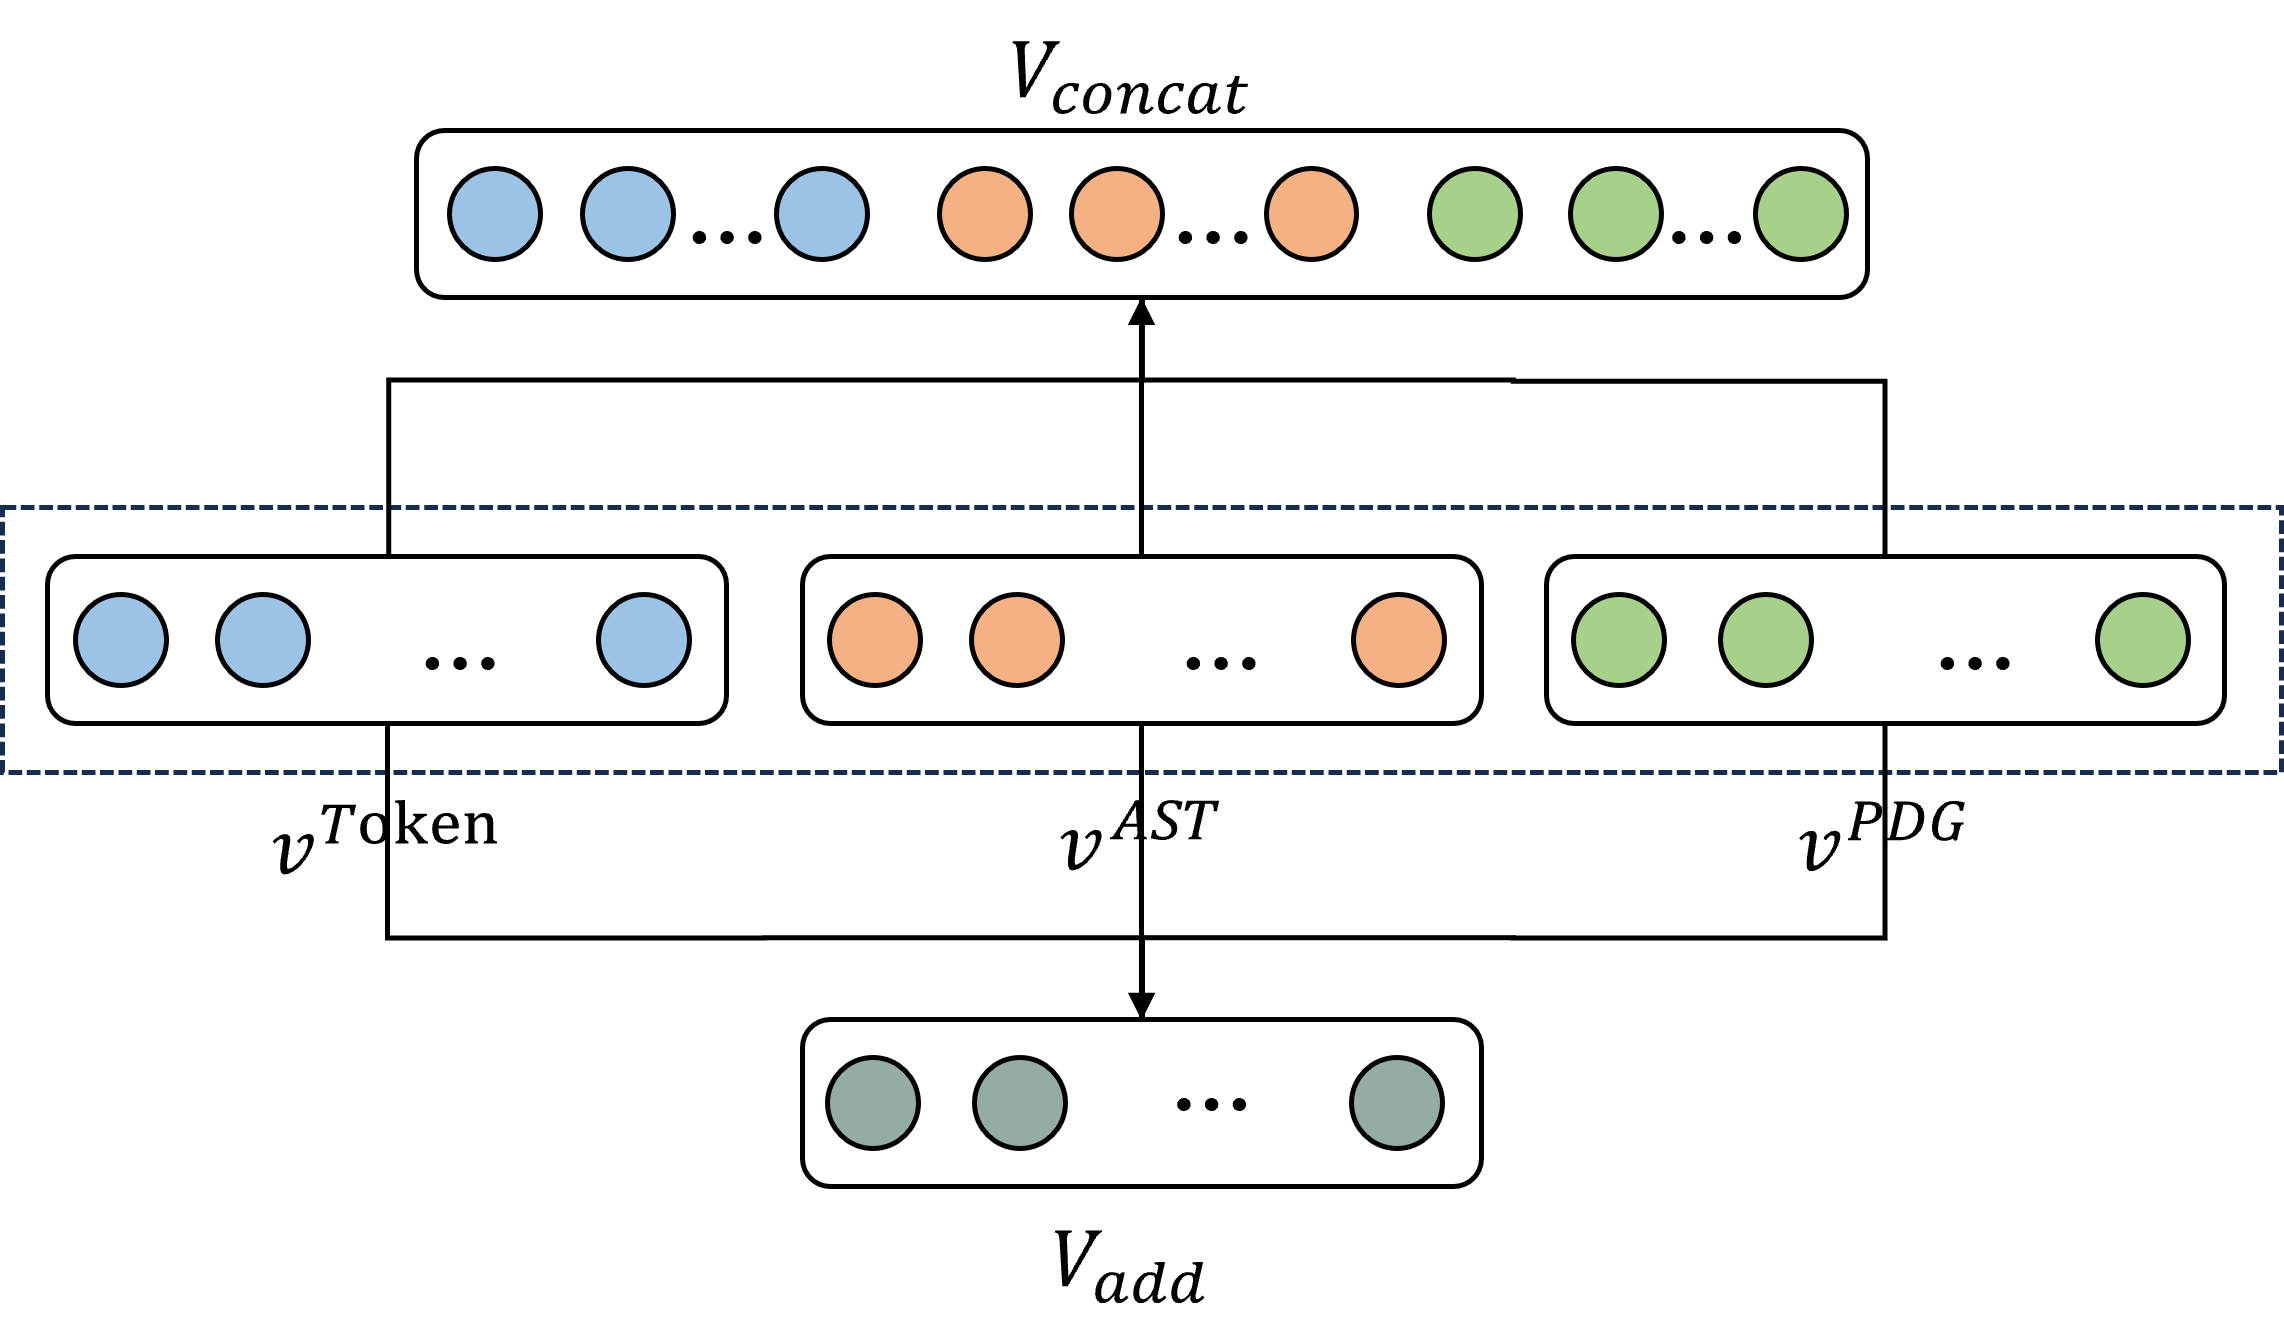
\includegraphics[width=0.55\textwidth]{figures/concat_add.png}
  \caption{特征融合方法}\label{fig:concat_add}
\end{figure}

其中特征连接Concat是指直接将两个特征张量在某个维度上连接在一起,生成一个更大的张量。例如两个输入特征x和y的维数若为p和q,输出特征z的维数为p+q。在连接时,采取串联策略,两个张量的维度必须保持一致。而特征加法Add是指将两个特征张量按照元素相加在一起,生成一个新的张量。采取并行策略,特征向量本身的维度并没有增加。上述两种融合方式可以用公式\ref{e6.1}表示:

\begin{equation}\label{e6.1}
  \begin{split}
    \tilde{V_{concat}} &= concat \left( V^{\text{Token}} , V^{\text{AST}} , V^{\text{PDG}}\right) \\
    \tilde{V_{add}} &= add \left( V^{\text{Token}} , V^{\text{AST}} , V^{\text{PDG}}\right) \\
    V &= W_{dt} \cdot \tilde{V} + b_{dt}
  \end{split}
\end{equation}

其中$V$表示最终的多维混合代码表示,$W_{dt}$在生成的多维混合表示中平衡属性特征、结构特征、语义特征的组成,而$b_{dt}$在训练模型时使模型偏向最终收敛。

\section{RLCCD框架验证}
本文的实验设计主要围绕以下5个方面的研究问题:

• RQ1:本文提出的预训练辅助模型策略是否优于基线方法?

• RQ2:本文提出的子树划分策略是否优于基线方法?

• RQ3:本文提出的图过滤策略能否优于基线方法?

• RQ4:本文提出的特征融合方法是否优于单个维度方法?

• RQ5:本文提出的多维源代码表征学习方法,与现有代码克隆检测工具相比表现如何?

在上述5个方向的研究问题中,RQ1是针对Token维度优化策略的评估,在\ref{sec:TokenExperiment}小节中已经给出;RQ2是针对抽象语法树维度优化策略的评估,在\ref{sec:ASTExperiment}小节中已经给出;RQ3是针对程序依赖图维度优化策略的评估,在\ref{sec:PDGExperiment}小节中已经给出;RQ4是针对基于多模态学习的特征融合方法进行评估;RQ5从整体工具有效性的角度开展评估。

\subsection{实验设置}

本章实验均在Ubuntu 16.04 LTS(64位)系统下进行,其系统硬件配置与\ref{subsec:Environment}所述相同。本实验选用JieBa分词获取代码的Token序列,使用代码分析工具Joern获取代码的抽象语法树、程序依赖图。代码克隆检测模型的开发过程中使用到的编程语言L:Python 3.6、深度学习框架Pytorch1.10、机器学习库Scilit-learn 0.19。同时,为了验证RLCCD的可行性与有效性,本章实验仍选用与前述\ref{subsec:Dataset}相同的数据集,并按照3:1:1的比例将其划分为训练集、测试集、验证集,所有实验在训练集上训练模型,并选择在验证集上产生最佳F1的参数来评估模型在测试集上的性能。

\subsection{对比工具}

为了更好地对比整个方法的实验效果,本文选取近几年来各个维度较为先进、经典开源的方法,并在相同数据集上进行了检测结果的对比,具体方法主要如表\ref{tab:tool}所示。

\begin{table}[htp]
  \centering
  \caption{代码克隆检测实验对比工具介绍} 
  \label{tab:tool}
  \renewcommand{\arraystretch}{1.1}
  \begin{tabular*}{0.8\textwidth}{@{\extracolsep{\fill}}cc}
  \toprule
    方法名称			&类型介绍		\\
  \midrule
  SourcererCC		 &基于Token的克隆检测方法 \\
  ASTNN			     &基于AST的克隆检测方法 \\
  CCSharp		     &基于PDG的克隆检测方法 \\
  SCDetector		 &基于Token、PDG的克隆检测方法 \\
  RLCCD(本文方法)	&基于Token、AST、PDG多种维度的克隆检测方法 \\
  \bottomrule
  \end{tabular*}
\end{table}

SourcererCC\cite{7886988}:SourcererCC是一种相对较新的基于token的克隆检测工具。该工具通过词袋模型,把收集的数据全部编码成词频信息,然后将代码行转换成一个由词频构成的向量,通过向量的比较获取相似度。

ASTNN\cite{8812062}:ASTNN是一种基于神经网络的源代码表示方法。它将整个抽象语法树AST分解成一系列小型语句子树,并通过捕获语句的词法和语法信息将语句子树分别编码为向量,最后采用了RNN模型生成代码片段的向量表示。ASTNN方法完整保留了抽象语法树的结构信息,能够检测到所有类型的代码克隆。

CCSharp\cite{9286111}:CCSharp是一种基于程序依赖图的代码克隆检测方法。它首先生成了源代码中函数级别的PDG,并对生成的图结构进行约简,随后进行特征向量的提取和过滤,最后应用Weisfeiler-Lehman图核算法进行图相似性比较找出代码克隆对。

SCDetector\cite{10.1145/3324884.3416562}:SCDetector一种是基于Token和图结合的方法。给定一个方法源代码,首先生成CFG,然后应用中心性分析将图转换为某些语义标记(即具有图细节的标记)。最后,这些语义标记被送到Siamese网络中,以训练模型并使用它来检测代码克隆对。

为了验证本文所提方法在克隆上的有效性,所有工具试实验结果均采用其参考文献中所提供的最好效果的参数配置,并统一在相同的实验数据集POJ104上进行对比实验。

\subsection{特征融合方法实验结果}

本节回答RQ4,本文提出的特征融合方法是否由于单个维度的表征方法?为了回答这个问题,本实验将Token、AST、PDG三个维度的最佳实验结果与多维融合方法Concat、Add进行对比。表\ref{tab:concat}展示了Token维度、树维度、图维度、采用Add方法融合三种维度、采用Concat方法融合三种维度共5种方法的准确率、召回率和F1得分。

\begin{table}[htp]
  \centering
  \caption{特征融合方法对实验结果的影响}
  \label{tab:concat}
  \begin{tabular*}{0.9\textwidth}{@{\extracolsep{\fill}}cccc}
  \toprule
    对比			& 准确率P(\%) & 召回率R(\%) & F1值(\%)  \\ 
  \midrule
    Token维度			   & 89.78	  & 95.62	  & 92.61	   \\  
    树维度		       & 92.75	  & 87.62	  & 90.11   \\ 
    图维度			     & 89.53		& 81.71		& 85.44   \\
    Add融合			     & 92.89		& 90.35		& 91.60   \\
    Concat融合     	 & 93.82		& 92.27		& 93.04  \\
  \bottomrule
  \end{tabular*}
\end{table}


基于对表\ref{tab:concat}数据的分析,可以得到以下结论:

(1)综合三种评估指标,基于多模态学习的特征融合方法的表现比单个维度的代码表征学习的表现优秀,其准确率、召回率、F1值均在92\%以上。说明基于多模态学习的特征融合方法可以利用数据之间的信息互补性,相较于单个维度,多维表征学习可以学习到更好的特征表示,从而有利于下游代码克隆检测任务的学习。

(2)Concat特征融合方法整体比Add融合方法表现优秀。深究其原因,Add特征融合相当于加入一种先验知识,对原始特征进行人为的特征融合。它描述的代码特征信息量增多,但维度本身并没有增加,当两个相加的特征向量不具备相同特征含义的时候,反而可能带来信息损失。而Concat特征融合是将三个张量拼接在一起,特征维度增加,每一特征下的信息并没有增加。这意味着Concat可以扩展特征的空间,让模型能够看到更多的信息和变化。通过将不同来源的特征拼接在一起,Concat可以促进特征之间的交互和整合,进一步提高模型的表现,使模型同时关注代码的局部和整体信息,因此具有更好的代码克隆检测能力。

(3)图维度的代码表征方法在代码克隆检测任务上的表现最差,三种指标均未超过90\%。深究其原因,可能是本文提出的基于图过滤的程序依赖图表征学习方法大大降低了图卷积神经网络模型的输入规模,数据量相比于基于Token的和基于树维度的表征方法少一个量级。当输入规模减少时,模型可能需要更长时间才能收敛到最优,同时模型可能无法充分学习数据的特征,影响下游任务表现。


\subsection{RLCCD性能评估实验结果}

本节回答RQ5,本文提出的RLCCD方法与现有代码克隆检测工具相比表现如何?为了回答这个问题,本实验RLCCD与Token维度方法SourcererCC、树维度方法ASTNN、图维度方法CCSharp、Token与图混合方法SCDetector进行对比,实验结果对比如表\ref{tab:RLCCD}所示。

\begin{table}[htp]
  \centering
  \caption{RLCCD性能评估实验结果}
  \label{tab:RLCCD}
  \begin{tabular*}{0.9\textwidth}{@{\extracolsep{\fill}}cccc}
  \toprule
    对比工具		& 准确率P(\%) & 召回率R(\%) & F1值(\%)  \\ 
  \midrule
    SourcererCC		& 11.23	  & 43.52		& 17.84 \\
    ASTNN			    & 87.92		& 95.47		& 91.54 \\
    CCSharp			  & 92.21	  & 52.13	  & 66.61 \\
    SCDetector		& 97.02	  & 81.05		& 88.32 \\
    RLCDD			    & 93.82		& 92.27		& 93.04  \\
  \bottomrule
  \end{tabular*}
\end{table}


基于对表\ref{tab:RLCCD}数据的分析,可以得到以下结论:

(1)本文提出的RLCCD在代码克隆检测任务中表现最好,其准确率、召回率、F1值均在92\%以上。说明RLCCD方法可以利用Token、AST、PDG三个维度数据之间的信息互补性,学习到更好的特征表示,代码信息利用率高,从而有利于提高下游代码克隆检测任务的精度。

(2)SourcererCC在代码克隆检测任务中表现最差。深究其原因,SourcererCC采用了一种优化的倒排索引方法来快速查询代码块中潜在的克隆,这种方法相对简单,主要反映了源代码的词汇级信息,但缺乏足够的代码的结构信息、语义信息。同时,由于代码关注词汇级别的相似度,因此会误报一些仅仅词汇相似但功能完全不同的代码克隆对,从而降低了检测的精度。

(3)ASTNN方法的召回率最高,达到了95.47\%。深究其原因,ASTNN同样采用了抽象语法树子树划分的方法,将每个大的AST语法树划分为语句树,通过捕获语句的词汇和句法知识将语句树编码为向量,与本文提出的RLCCD方法不同,ASTNN直接使用了基于递归神经网络RvNN的语句编码器学习语句的向量表示,使其能够适应不同大小和形状的树状数据,不必局限于数据的固定树状结构,具有很好的灵活性。ASTNN通过递归的方式将网络应用于数据的不同层次,从而捕捉复杂的层次结构和依赖关系,面向下游代码克隆检测任务的召回率达到最高。

(4)CCSharp方法的召回率相较于准确率表现很差,只有52.13\%。深究其原因,CCSharp是一种基于Weisfeiler-Lehman图核算法的代码克隆检测方法,其迭代过程中过于关注图结构信息,反而忽略了节点自身的特征信息,同时对迭代次数敏感,次数过少无法充分捕获图的结构信息。

(5)SCDetector方法的准确率最高,达到了97.02\%。说明多个维度的代码特征融合相较于单个维度,正确识别代码克隆对的能力优秀。深究其原因,SCDetector融合了Token和图两种不同层次的代码表示方法,从而能够同时捕获代码在词汇级别和结构级别上的相似性。因此,面对代码片段存在词汇上相似,或者结构上相似但在词汇上有所变化的情况,SCDetector依旧可以有效识别。

\section{本章小结}
本章节主要对RLCCD框架中基于多模态学习的特征融合方法进行了介绍,然后进行了实验验证。首先介绍了两种特征融合方法:Add、Concat,然后介绍了实验设置和对比工具,通过单个维度与多维源代码表征学习方法RLCCD的对比实验证明了RLCCD的有效性,最后通过将RLCCD与另外4种代码克隆检测方法进行了对比实验,证明了RLCCD具有较好的性能表现。



